% Dataset stats: HMDf-IAI
\begin{figure}[ht]
%\captionsetup[subfigure]{labelformat=empty}
\begin{center}
\subfloat[\Gls{teental}]{\label{fig:dstats:HMDf:IAI:teen}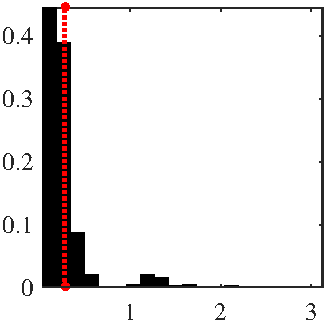
\includegraphics[scale=1]{dstats/HMDf-teen-IAI.pdf}} \hspace{0.5cm} 
\subfloat[\Gls{ektal}]{\label{fig:dstats:HMDf:IAI:ek}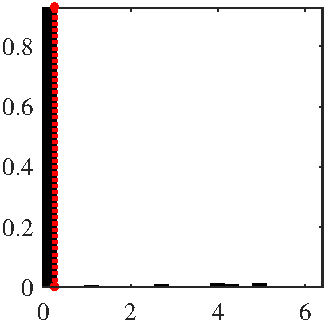
\includegraphics[scale=1]{dstats/HMDf-ek-IAI.pdf}} \\ 
\subfloat[\Gls{jhaptal}]{\label{fig:dstats:HMDf:IAI:jhap}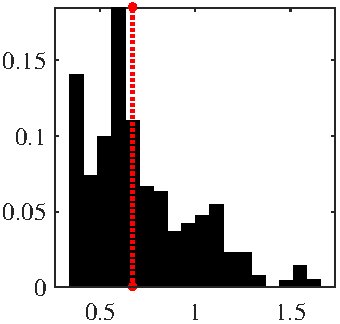
\includegraphics[scale=1]{dstats/HMDf-jhap-IAI.pdf}} \hspace{0.5cm} 
\subfloat[\Gls{rupak}]{\label{fig:dstats:HMDf:IAI:rupak}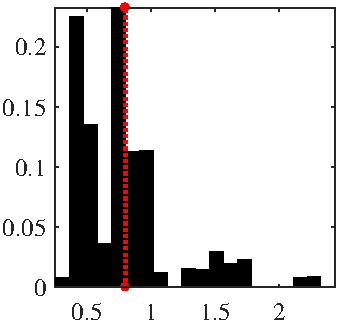
\includegraphics[scale=1]{dstats/HMDf-rupak-IAI.pdf}} \\ 
\caption[HMDf-IAI]{HMDf-IAI}\label{fig:dstats:HMDf:IAI}
\end{center}
\end{figure}


% Dataset stats: HMDf-IAInorm
\begin{figure}[ht]
%\captionsetup[subfigure]{labelformat=empty}
\begin{center}
\subfloat[\Gls{teental}]{\label{fig:dstats:HMDf:IAInorm:teen}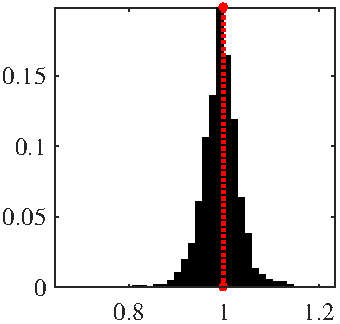
\includegraphics[scale=1]{dstats/HMDf-teen-IAInorm.pdf}} \hspace{0.5cm} 
\subfloat[\Gls{ektal}]{\label{fig:dstats:HMDf:IAInorm:ek}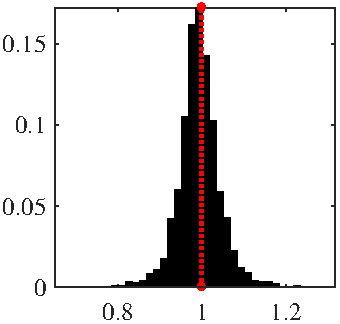
\includegraphics[scale=1]{dstats/HMDf-ek-IAInorm.pdf}} \\ 
\subfloat[\Gls{jhaptal}]{\label{fig:dstats:HMDf:IAInorm:jhap}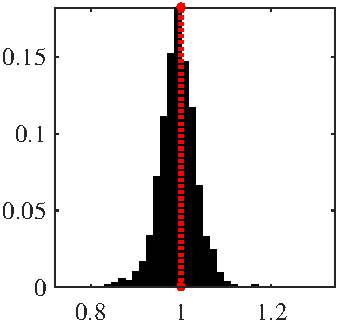
\includegraphics[scale=1]{dstats/HMDf-jhap-IAInorm.pdf}} \hspace{0.5cm} 
\subfloat[\Gls{rupak}]{\label{fig:dstats:HMDf:IAInorm:rupak}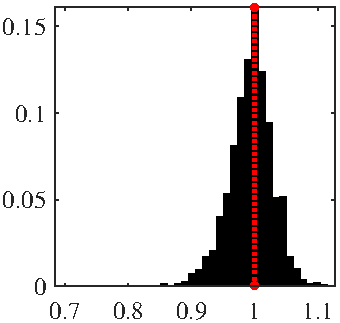
\includegraphics[scale=1]{dstats/HMDf-rupak-IAInorm.pdf}} \\ 
\caption[HMDf-IAInorm]{HMDf-IAInorm}\label{fig:dstats:HMDf:IAInorm}
\end{center}
\end{figure}


% Dataset stats: HMDf-ISI
\begin{figure}[ht]
%\captionsetup[subfigure]{labelformat=empty}
\begin{center}
\subfloat[\Gls{teental}]{\label{fig:dstats:HMDf:ISI:teen}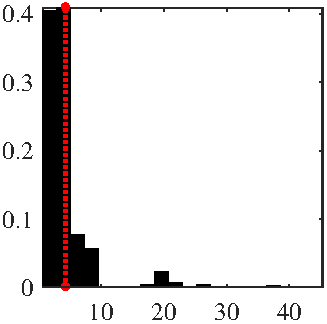
\includegraphics[scale=1]{dstats/HMDf-teen-ISI.pdf}} \hspace{0.5cm} 
\subfloat[\Gls{ektal}]{\label{fig:dstats:HMDf:ISI:ek}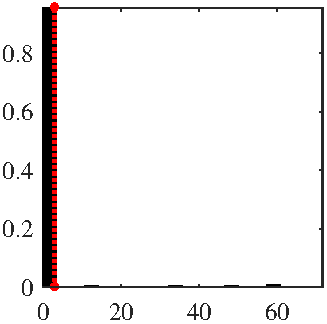
\includegraphics[scale=1]{dstats/HMDf-ek-ISI.pdf}} \\ 
\subfloat[\Gls{jhaptal}]{\label{fig:dstats:HMDf:ISI:jhap}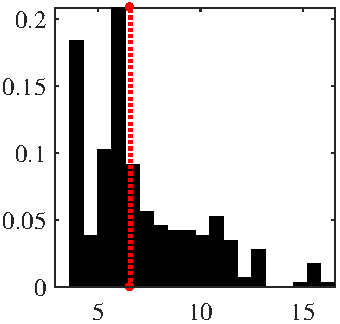
\includegraphics[scale=1]{dstats/HMDf-jhap-ISI.pdf}} \hspace{0.5cm} 
\subfloat[\Gls{rupak}]{\label{fig:dstats:HMDf:ISI:rupak}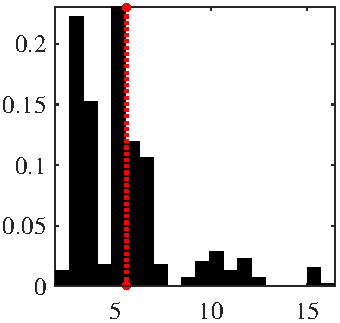
\includegraphics[scale=1]{dstats/HMDf-rupak-ISI.pdf}} \\ 
\caption[HMDf-ISI]{HMDf-ISI}\label{fig:dstats:HMDf:ISI}
\end{center}
\end{figure}


% Dataset stats: HMDf-ISInorm
\begin{figure}[ht]
%\captionsetup[subfigure]{labelformat=empty}
\begin{center}
\subfloat[\Gls{teental}]{\label{fig:dstats:HMDf:ISInorm:teen}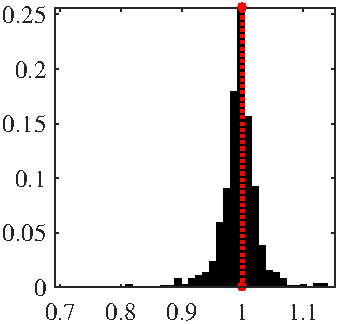
\includegraphics[scale=1]{dstats/HMDf-teen-ISInorm.pdf}} \hspace{0.5cm} 
\subfloat[\Gls{ektal}]{\label{fig:dstats:HMDf:ISInorm:ek}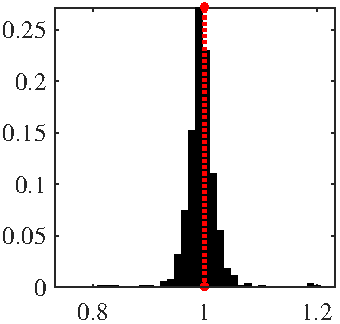
\includegraphics[scale=1]{dstats/HMDf-ek-ISInorm.pdf}} \\ 
\subfloat[\Gls{jhaptal}]{\label{fig:dstats:HMDf:ISInorm:jhap}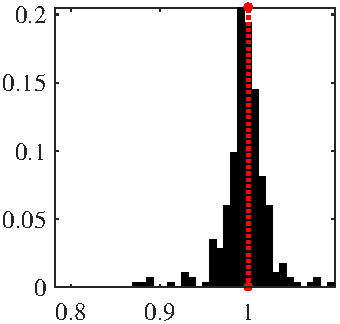
\includegraphics[scale=1]{dstats/HMDf-jhap-ISInorm.pdf}} \hspace{0.5cm} 
\subfloat[\Gls{rupak}]{\label{fig:dstats:HMDf:ISInorm:rupak}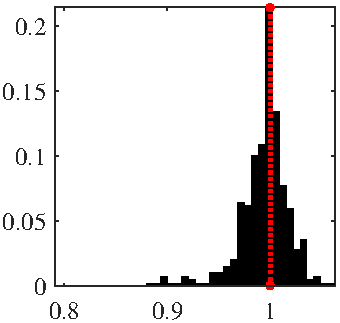
\includegraphics[scale=1]{dstats/HMDf-rupak-ISInorm.pdf}} \\ 
\caption[HMDf-ISInorm]{HMDf-ISInorm}\label{fig:dstats:HMDf:ISInorm}
\end{center}
\end{figure}

